\documentclass[11pt,a4paper]{article}

% ---------- Packages ----------
\usepackage[utf8]{inputenc}
\usepackage[T1]{fontenc}
\usepackage[margin=2.4cm]{geometry}
\usepackage{amsmath,amssymb,amsthm}
\usepackage{graphicx}
\usepackage{booktabs}
\usepackage{multirow}
\usepackage{array}
\usepackage{caption}
\usepackage{subcaption}
\usepackage{xcolor}
\usepackage{hyperref}
\usepackage[protrusion=true,expansion=false]{microtype}
\usepackage{enumitem}
\usepackage{listings}
\usepackage{titlesec}
\usepackage{fancyhdr}

% ---------- Hyperref ----------
\hypersetup{
  colorlinks=true,
  linkcolor=black!70!blue,
  urlcolor=blue!60!black,
  citecolor=black!70!blue,
}

% ---------- Headings ----------
\titleformat{\section}{\large\bfseries}{\thesection.}{0.6em}{}
\titleformat{\subsection}{\normalsize\bfseries}{\thesubsection}{0.5em}{}
\titlespacing*{\section}{0pt}{1.0em}{0.4em}
\titlespacing*{\subsection}{0pt}{0.7em}{0.2em}

\setlength{\parindent}{0pt}
\setlength{\parskip}{0.4em}
\captionsetup{font=small,labelfont=bf,skip=4pt}

% ---------- Listings ----------
\definecolor{codegray}{rgb}{0.45,0.45,0.45}
\lstset{
  basicstyle=\ttfamily\footnotesize,
  commentstyle=\color{codegray},
  keywordstyle=\color{blue!70!black},
  showstringspaces=false,
  breaklines=true,
  frame=none,
}

% ---------- Custom colours ----------
\definecolor{navyblue}{RGB}{31,57,99}
\definecolor{crimson}{RGB}{192,0,0}
\definecolor{steelblue}{RGB}{70,130,180}

% ---------- Title block ----------
\title{\vspace{-1.5em}\textbf{Mortgage Prepayment Risk Modeling:\\
From Kaplan--Meier to Deep Survival Analysis}\\[0.3em]
\large IR\&C Assignment 3 --- Spring 2026}
\author{Kassziopeia\\\small MTH 9877 --- Interest Rate and Credit Models, Baruch College}
\date{May 2026}

% ---------- Document ----------
\begin{document}
\maketitle
\vspace{-1.2em}

% =================================================================
\section{Introduction}
% =================================================================

Mortgage prepayment and default are the two primary sources of duration
and credit risk in agency mortgage-backed securities (MBS). A borrower
prepays by refinancing at a lower rate, selling the property, or paying
off the loan; a borrower defaults by ceasing payments and eventually
losing the property through foreclosure or short sale. From a fixed-income
perspective, prepayment shortens duration when rates fall (negative
convexity) while default imposes credit loss.

Standard survival analysis treats all exits as realizations of a single
event. In mortgage modelling this is incorrect: prepayment and default are
\emph{competing risks} --- the occurrence of one permanently prevents the
other. This report documents the full competing-risks survival analysis
conducted on the \textbf{Freddie Mac Single-Family Loan-Level Dataset}
(34 million 30-year fixed-rate mortgages, 1999--2023), covering:

\begin{itemize}[leftmargin=1.4em,itemsep=2pt]
  \item \textbf{E(i)} Competing-risks framework: EDA, Aalen--Johansen CIF,
        KM bias, stratified CIF, cause-specific Cox, Fine--Gray.
  \item \textbf{E(ii)} Time-dependent covariates via Andersen--Gill
        counting-process Cox.
  \item \textbf{E(iii)} Neural survival models (DeepHit architecture).
  \item \textbf{E(iv)} Scenario analysis: prepayment sensitivity to
        $\pm200\,\text{bp}$ rate shocks.
\end{itemize}

% =================================================================
\section{Data and Methodology}
% =================================================================

\subsection{Dataset}

The analysis uses three datasets constructed from Freddie Mac public
release files:

\begin{center}
\begin{tabular}{llr}
\toprule
\textbf{File} & \textbf{Contents} & \textbf{Rows} \\
\midrule
\texttt{survival\_loans.parquet}  & One row per FRM-360 loan  & 34{,}013{,}469 \\
\texttt{macro\_monthly.parquet}   & Monthly macro series (FRED) & $\sim$312 \\
\texttt{panel\_monthly.parquet}   & Loan $\times$ month panel & $\sim$93\,M \\
\bottomrule
\end{tabular}
\end{center}

\textbf{Filter}: \texttt{AmortizationType = `FRM'} and
\texttt{OriginalLoanTerm = 360}. Origination years 1999--2023.
Macro covariates: 30-year mortgage rate (MORTGAGE30US), unemployment
rate (UNRATE), CPI year-on-year (CPIAUCSL), and HPI year-on-year
(CSUSHPISA), sourced from FRED.

\subsection{Event definitions}

\begin{itemize}[leftmargin=1.4em,itemsep=1pt]
  \item \textbf{Prepayment} (cause 1): \texttt{ZeroBalanceCode = 1}
        (voluntary payoff or refinance).
  \item \textbf{Default} (cause 2): \texttt{ZeroBalanceCode} $\in$
        \{2, 3, 9\} (third-party sale, short sale, REO).
  \item \textbf{Censored}: loan still active at analysis date or exited
        for other reasons (repurchase, note sale).
\end{itemize}

\subsection{Sampling strategy}

Survival and Cox models use a \textbf{100\,K stratified subsample}
(proportional by vintage year) drawn from the 34\,M loan file.
The Andersen--Gill TV-Cox uses 10\,K loans from the monthly panel.

% =================================================================
\section{E(i)(a) --- Exploratory Data Analysis}
% =================================================================

\begin{figure}[h]
  \centering
  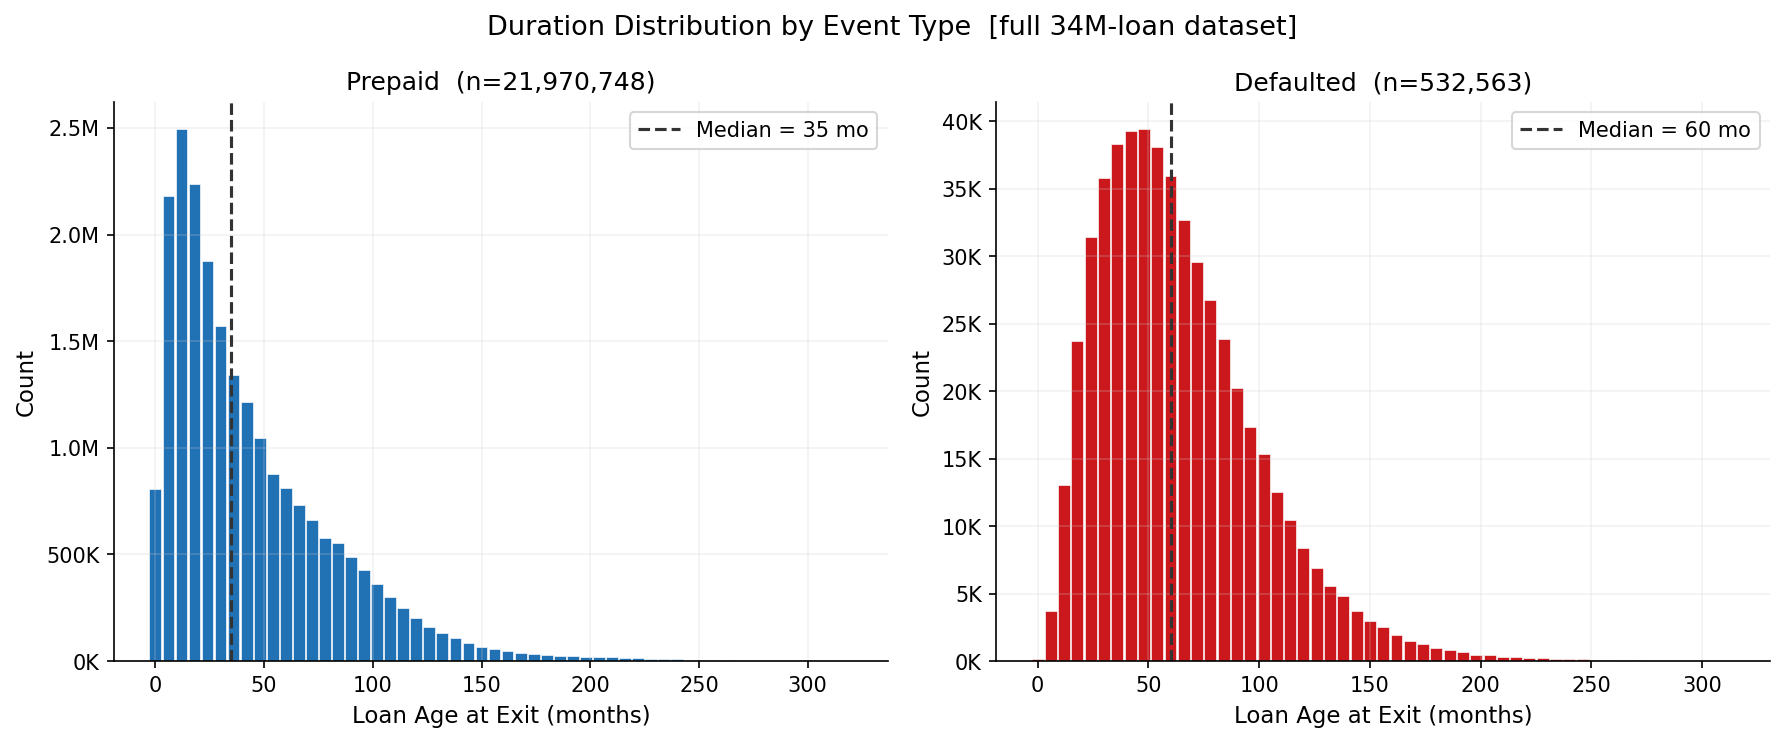
\includegraphics[width=\linewidth]{processed/E1_eda_duration}
  \caption{Duration distributions by event type across the full
    34\,M-loan dataset. Prepaid loans exit at a median of 35 months
    (rate-option exercise); defaults cluster around a median of 60
    months (gradual financial deterioration); censored loans have a
    median of 30 months (recent originations still active).}
  \label{fig:eda_duration}
\end{figure}

\begin{figure}[h]
  \centering
  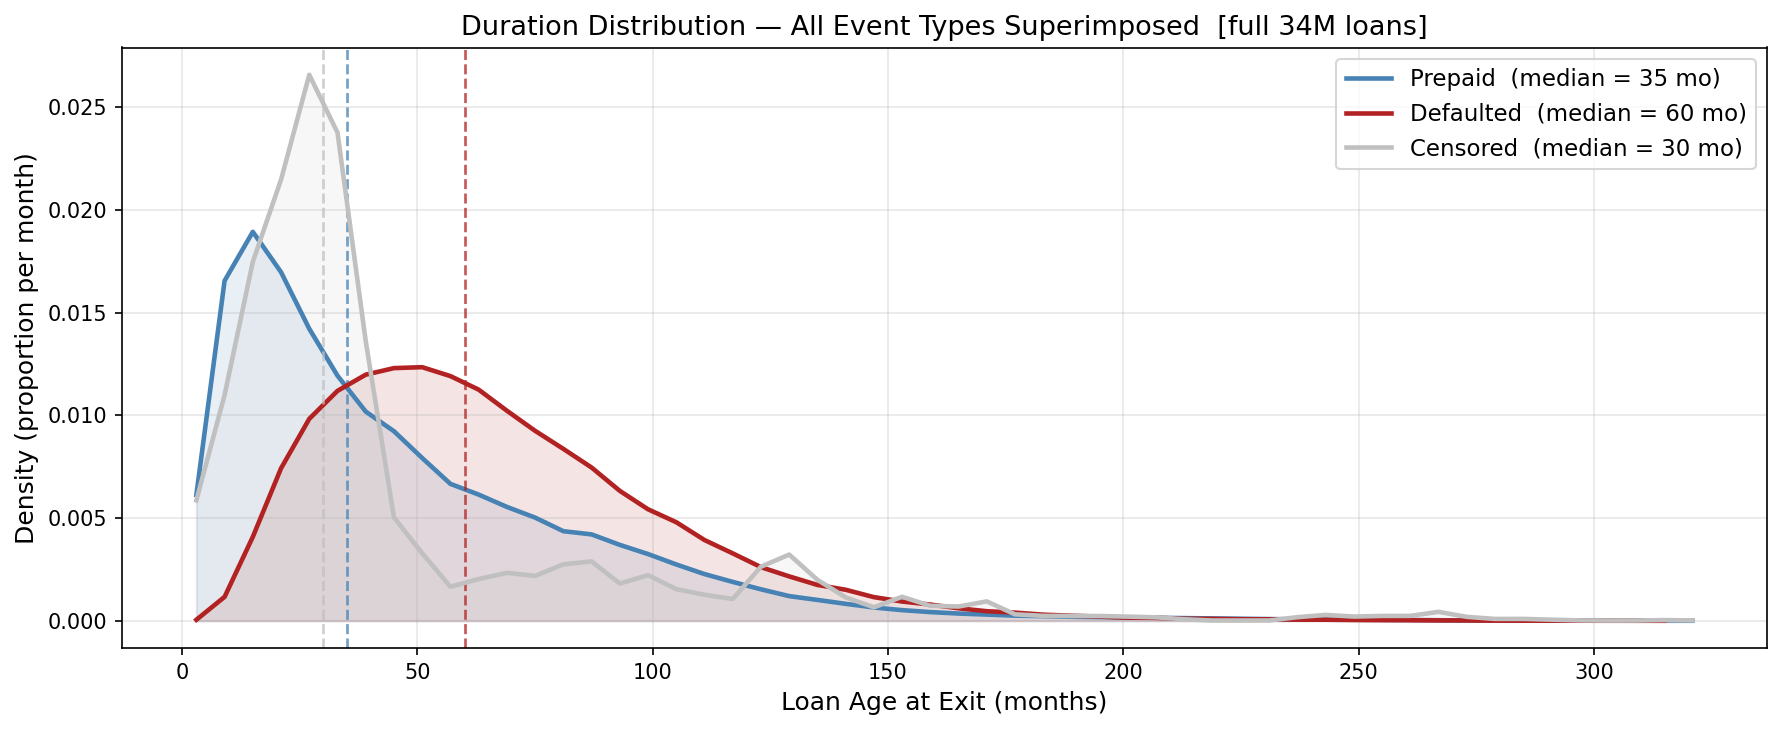
\includegraphics[width=\linewidth]{processed/E1_eda_duration_overlay}
  \caption{Superimposed duration density curves, normalised within each
    event type (proportion per month). Dashed vertical lines mark group
    medians. Prepayment density peaks sharply near month~15 and decays
    rapidly (burnout); default density is flatter and right-shifted,
    peaking near month~60; censored loans concentrate in the first
    30~months reflecting recent originations still in their early
    performance window.}
  \label{fig:eda_duration_overlay}
\end{figure}

Table~\ref{tab:eda_summary} summarises the three groups across the
full 34\,M-loan dataset.

\begin{table}[h]
\centering
\caption{Summary statistics by event type (full 34\,M-loan dataset).}
\label{tab:eda_summary}
\small
\begin{tabular}{lrrrrrrrr}
\toprule
\textbf{Event} & \textbf{N} & \textbf{Share} & \textbf{Med\,dur} &
\textbf{FICO} & \textbf{LTV} & \textbf{Rate} & \textbf{DTI} &
\textbf{UPB\,\$K} \\
\midrule
Prepaid   & 21{,}970{,}748 & 64.6\% & 35\,mo & 739 & 73.9\% & 5.39\% & 34.2 & 212 \\
Defaulted &    532{,}563   &  1.6\% & 60\,mo & 695 & 82.5\% & 6.24\% & 38.8 & 170 \\
Censored  & 11{,}510{,}158 & 33.8\% & 30\,mo & 756 & 71.2\% & 4.37\% & 33.1 & 285 \\
\bottomrule
\end{tabular}
\end{table}

\begin{figure}[h]
  \centering
  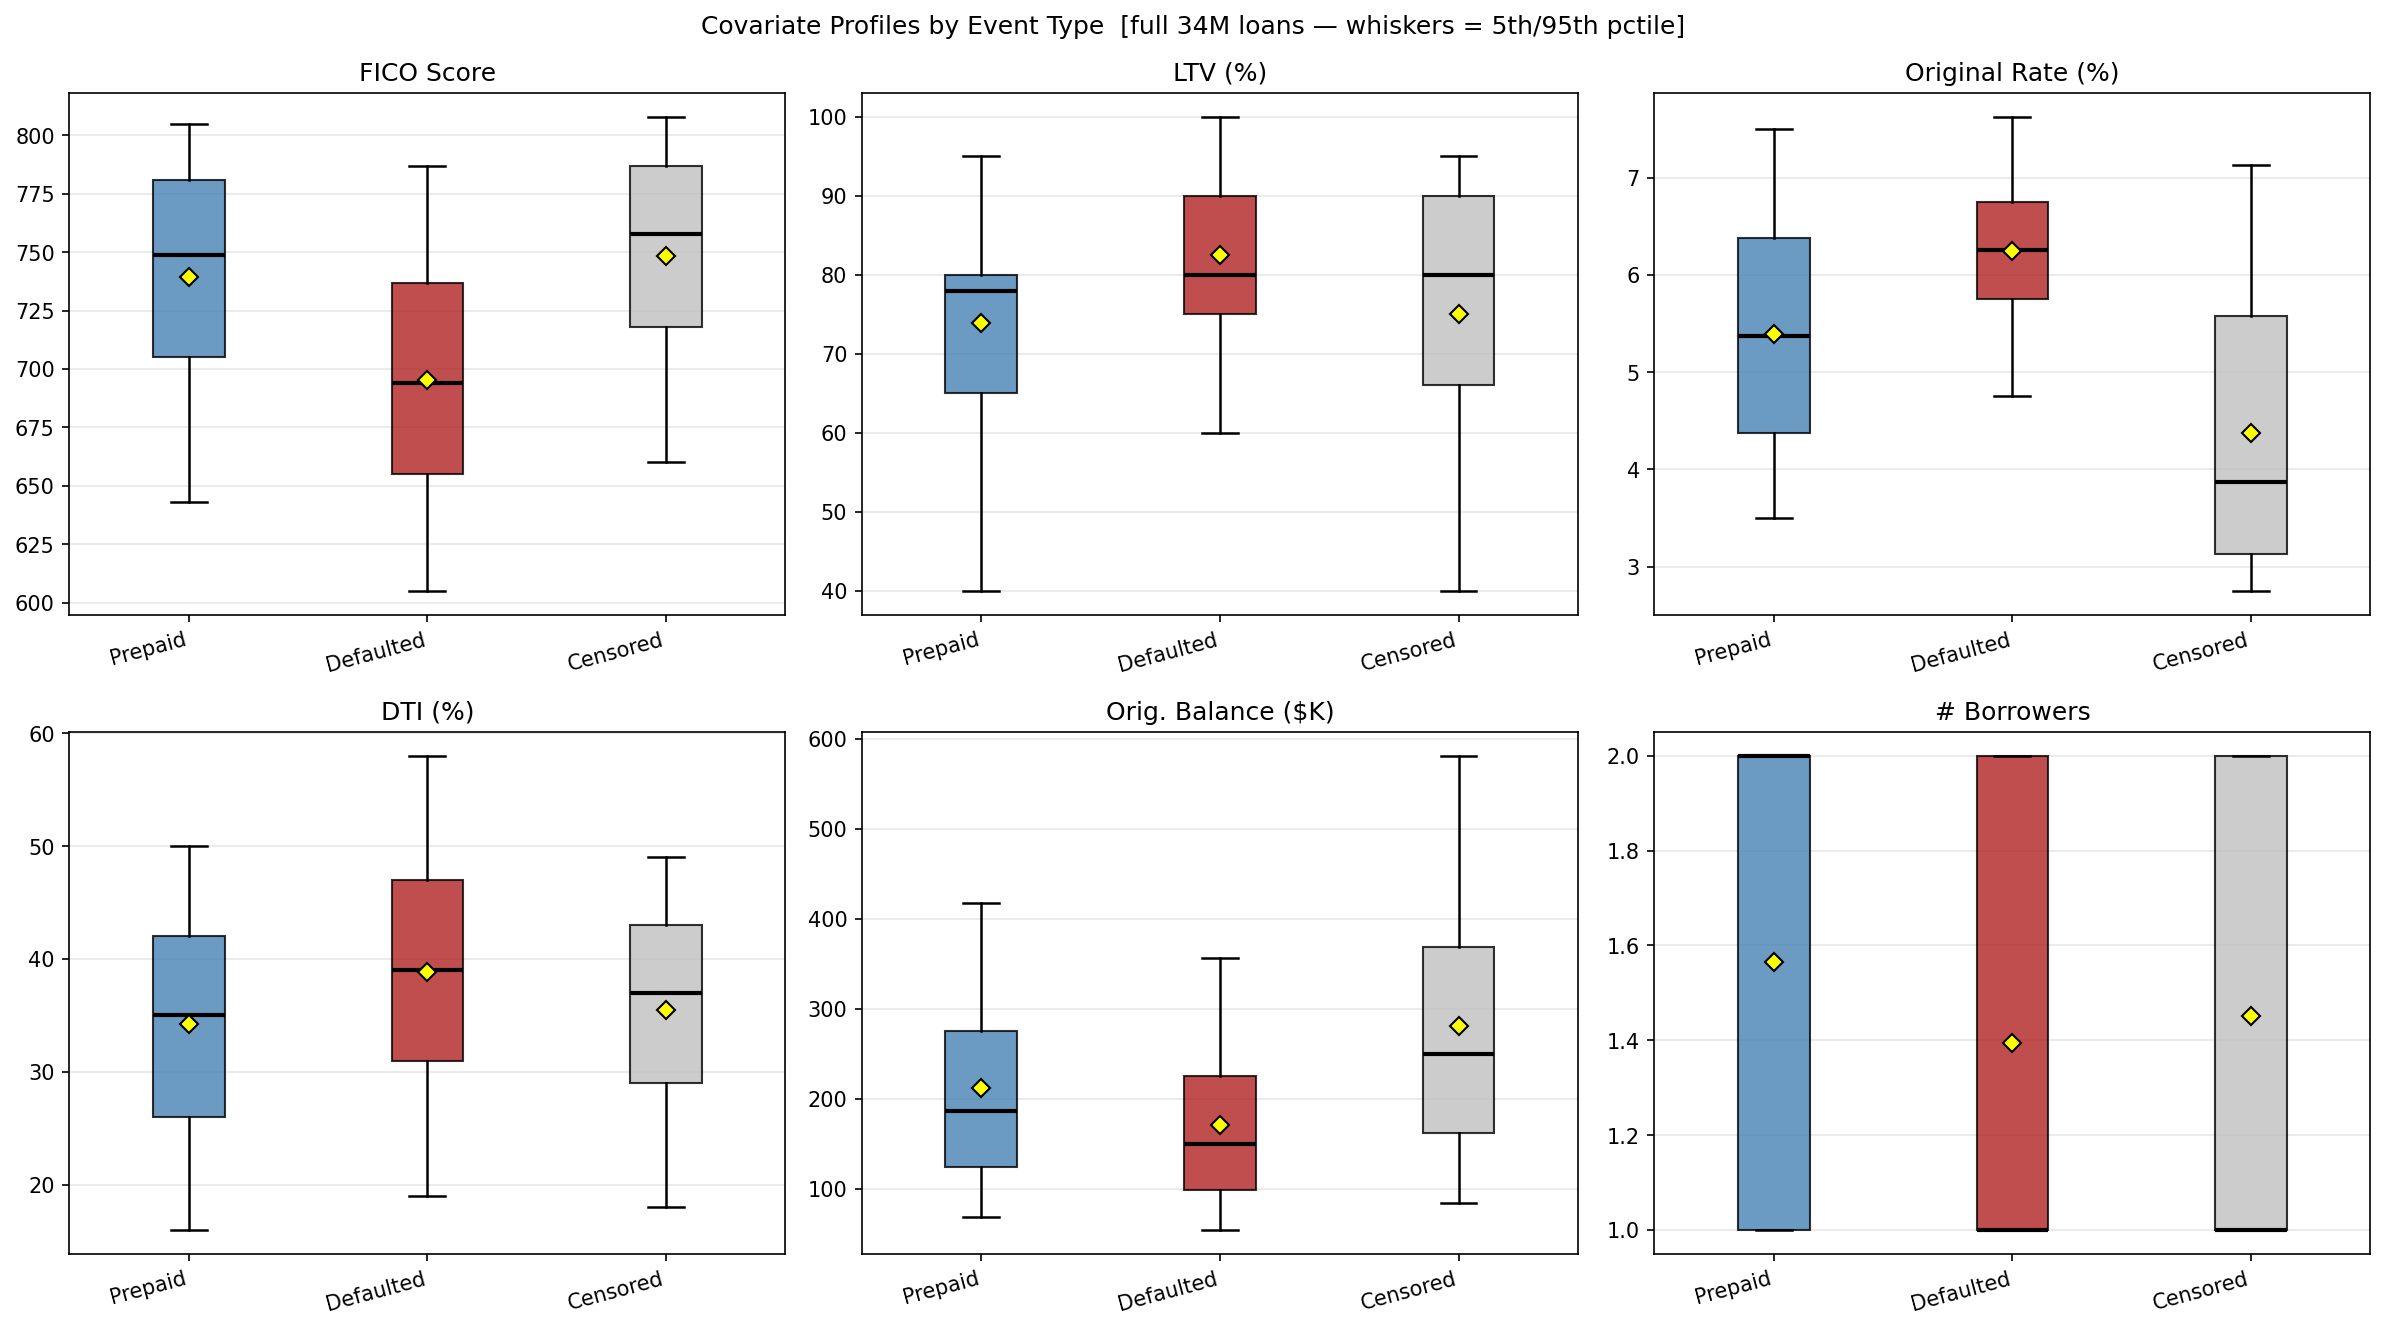
\includegraphics[width=\linewidth]{processed/E1_eda_covariates}
  \caption{Covariate profiles by event type (six features). Whiskers
    span the 5th--95th percentile. Defaulted borrowers show lower
    FICO ($-44$\,pts), higher LTV ($+8.6$\,pp), higher rate
    ($+0.85$\,pp), and higher DTI ($+4.6$\,pp) relative to prepaid.
    Censored loans have the largest balances (\$285\,K median), consistent
    with recent high-price originations that are rate-locked.}
  \label{fig:eda_covariates}
\end{figure}

\begin{figure}[h]
  \centering
  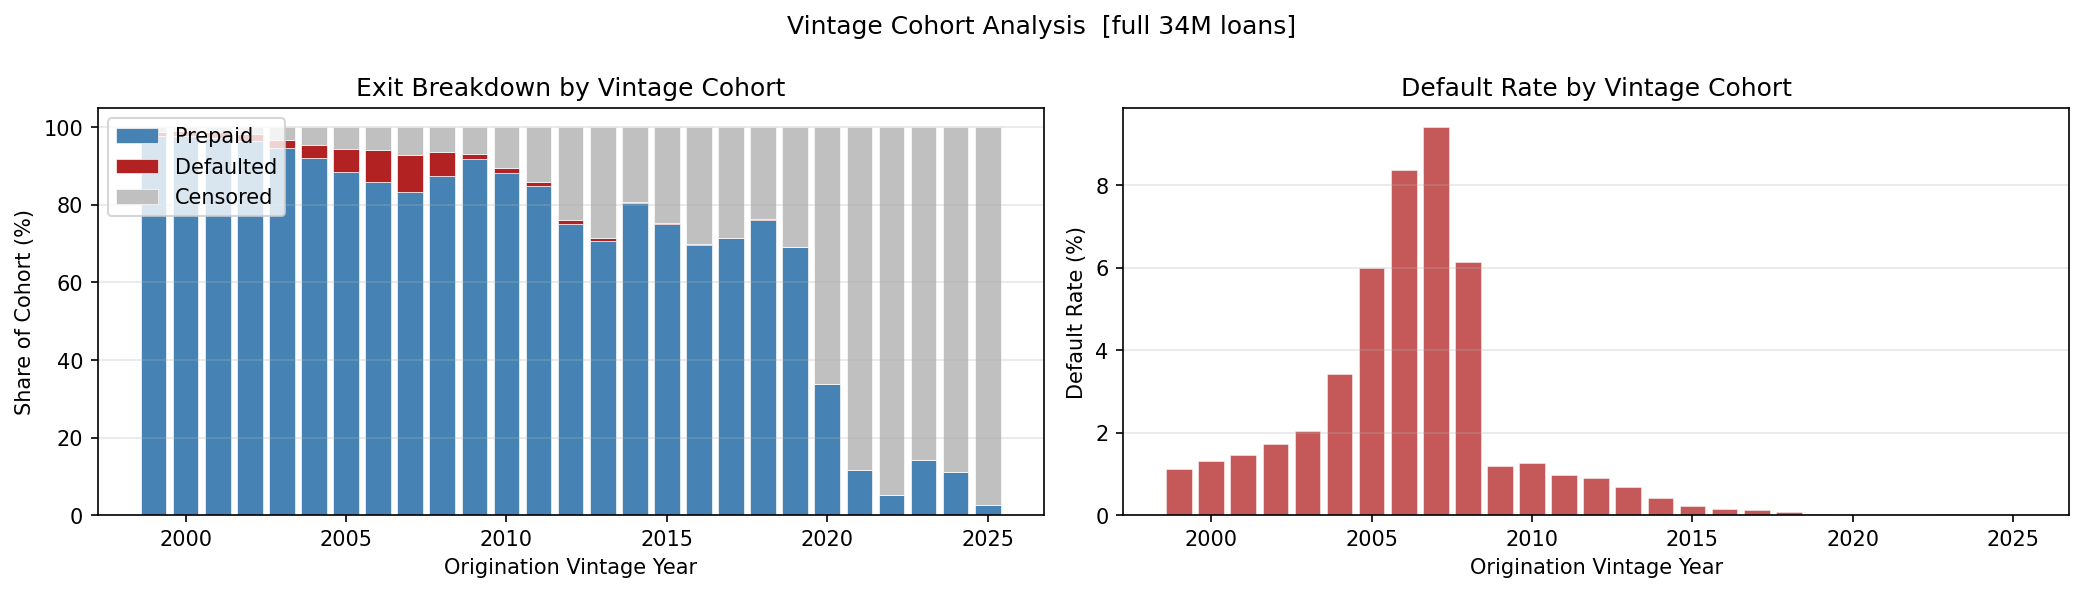
\includegraphics[width=\linewidth]{processed/E1_eda_vintage}
  \caption{Vintage cohort analysis. Left: stacked exit breakdown.
    Right: default rate by origination year. The 2007 cohort reaches
    $\approx 8.5\%$ default rate --- 6$\times$ the long-run average of
    $\approx 1.4\%$ --- driven by GFC-era underwriting. Post-2013
    cohorts approach zero default due to tighter standards. Post-2020
    cohorts show a large censored share reflecting rate lock-in.}
  \label{fig:eda_vintage}
\end{figure}

\begin{figure}[h]
  \centering
  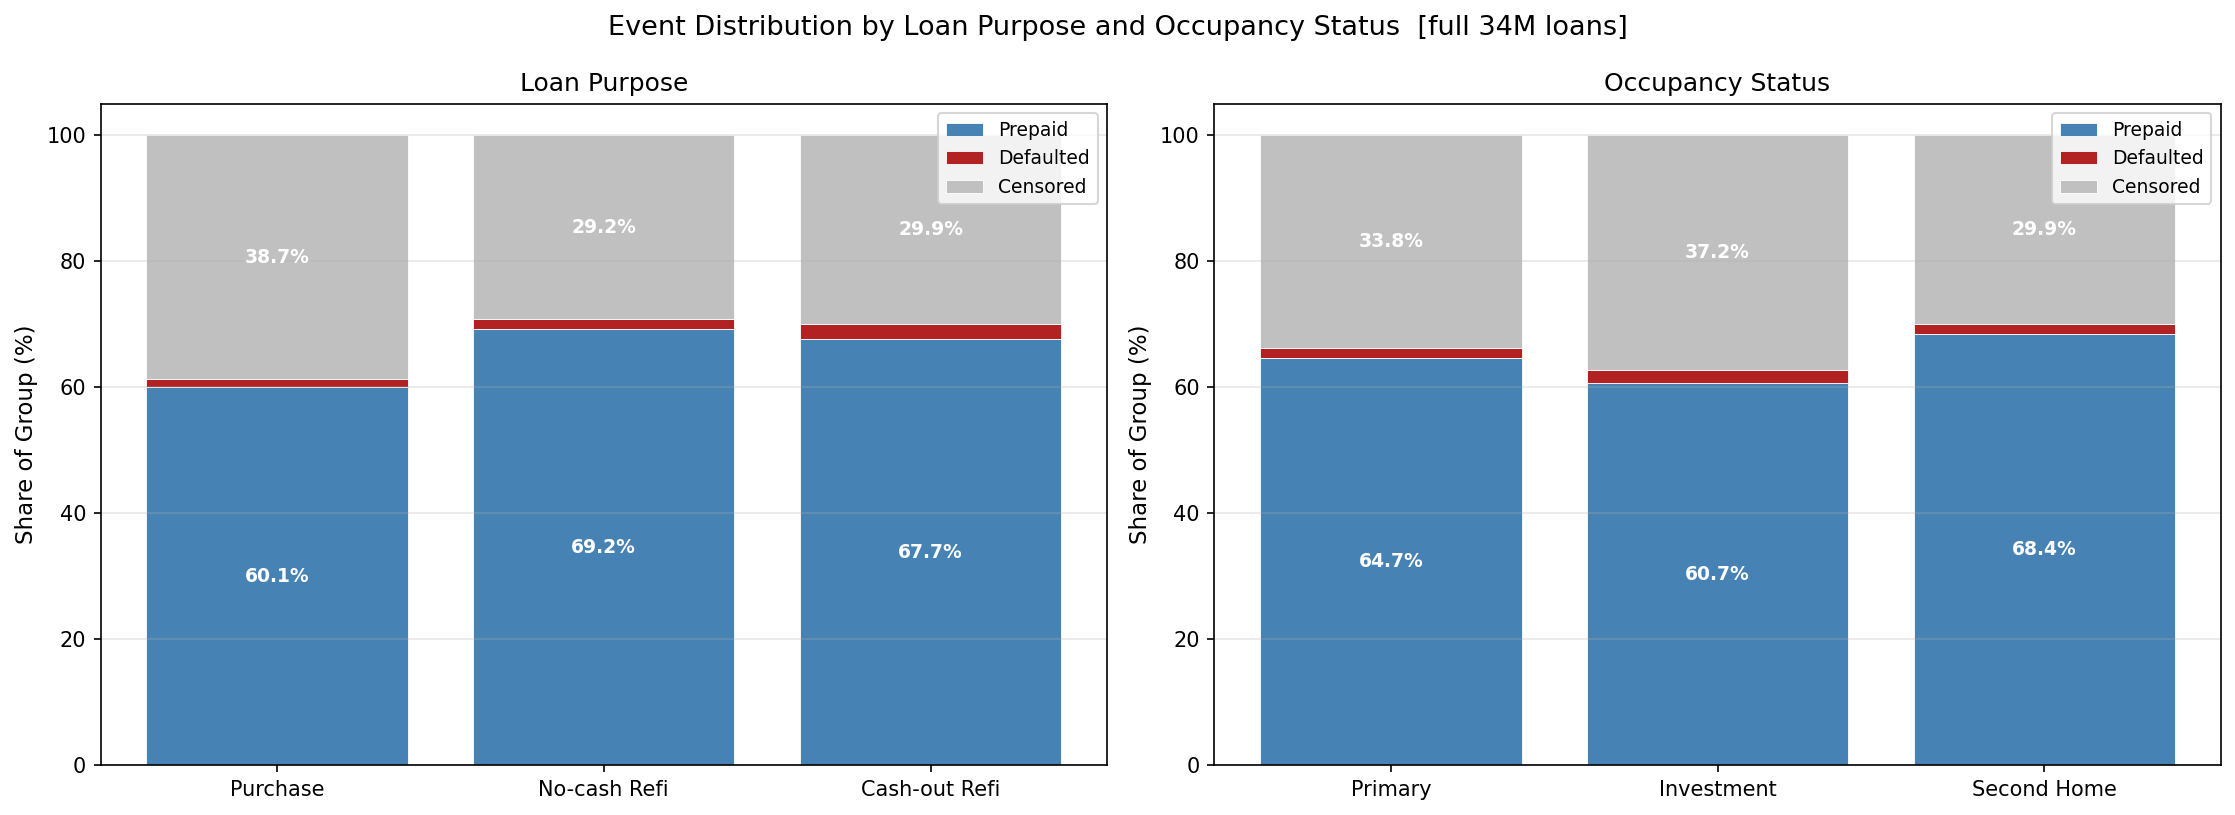
\includegraphics[width=\linewidth]{processed/E1_eda_categorical}
  \caption{Exit breakdown by loan purpose and occupancy status. Cash-out
    refinances show a modestly higher default share. Investment
    properties exhibit the highest default rate among occupancy
    categories ($\approx 3.2\%$), consistent with strategic default
    behaviour absent in primary-residence borrowers.}
  \label{fig:eda_cat}
\end{figure}

\subsection{Hazard intensity}

Figure~\ref{fig:hazard_overall} shows the cause-specific Nelson--Aalen
smoothed hazard $h(t)$ estimated from the 100\,K subsample. The
prepayment hazard peaks at $t \approx 30$--$40$ months then decays
sharply --- the \emph{burnout effect}: the most rate-sensitive borrowers
exit early, leaving a survivor pool with low refinancing propensity.
The default hazard rises slowly and plateaus, consistent with gradual
financial stress rather than a discrete shock.

\begin{figure}[h]
  \centering
  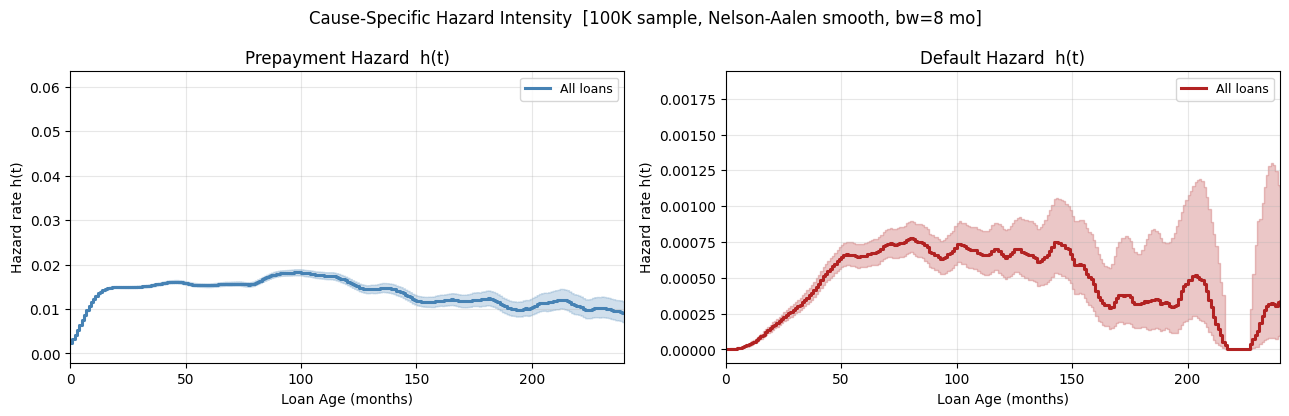
\includegraphics[width=\linewidth]{processed/E1_hazard_overall}
  \caption{Cause-specific hazard intensity $h(t)$ for prepayment
    (left) and default (right). Estimated via Nelson--Aalen with
    kernel bandwidth $= 8$\,months on the 100\,K stratified subsample.}
  \label{fig:hazard_overall}
\end{figure}

\begin{figure}[h]
  \centering
  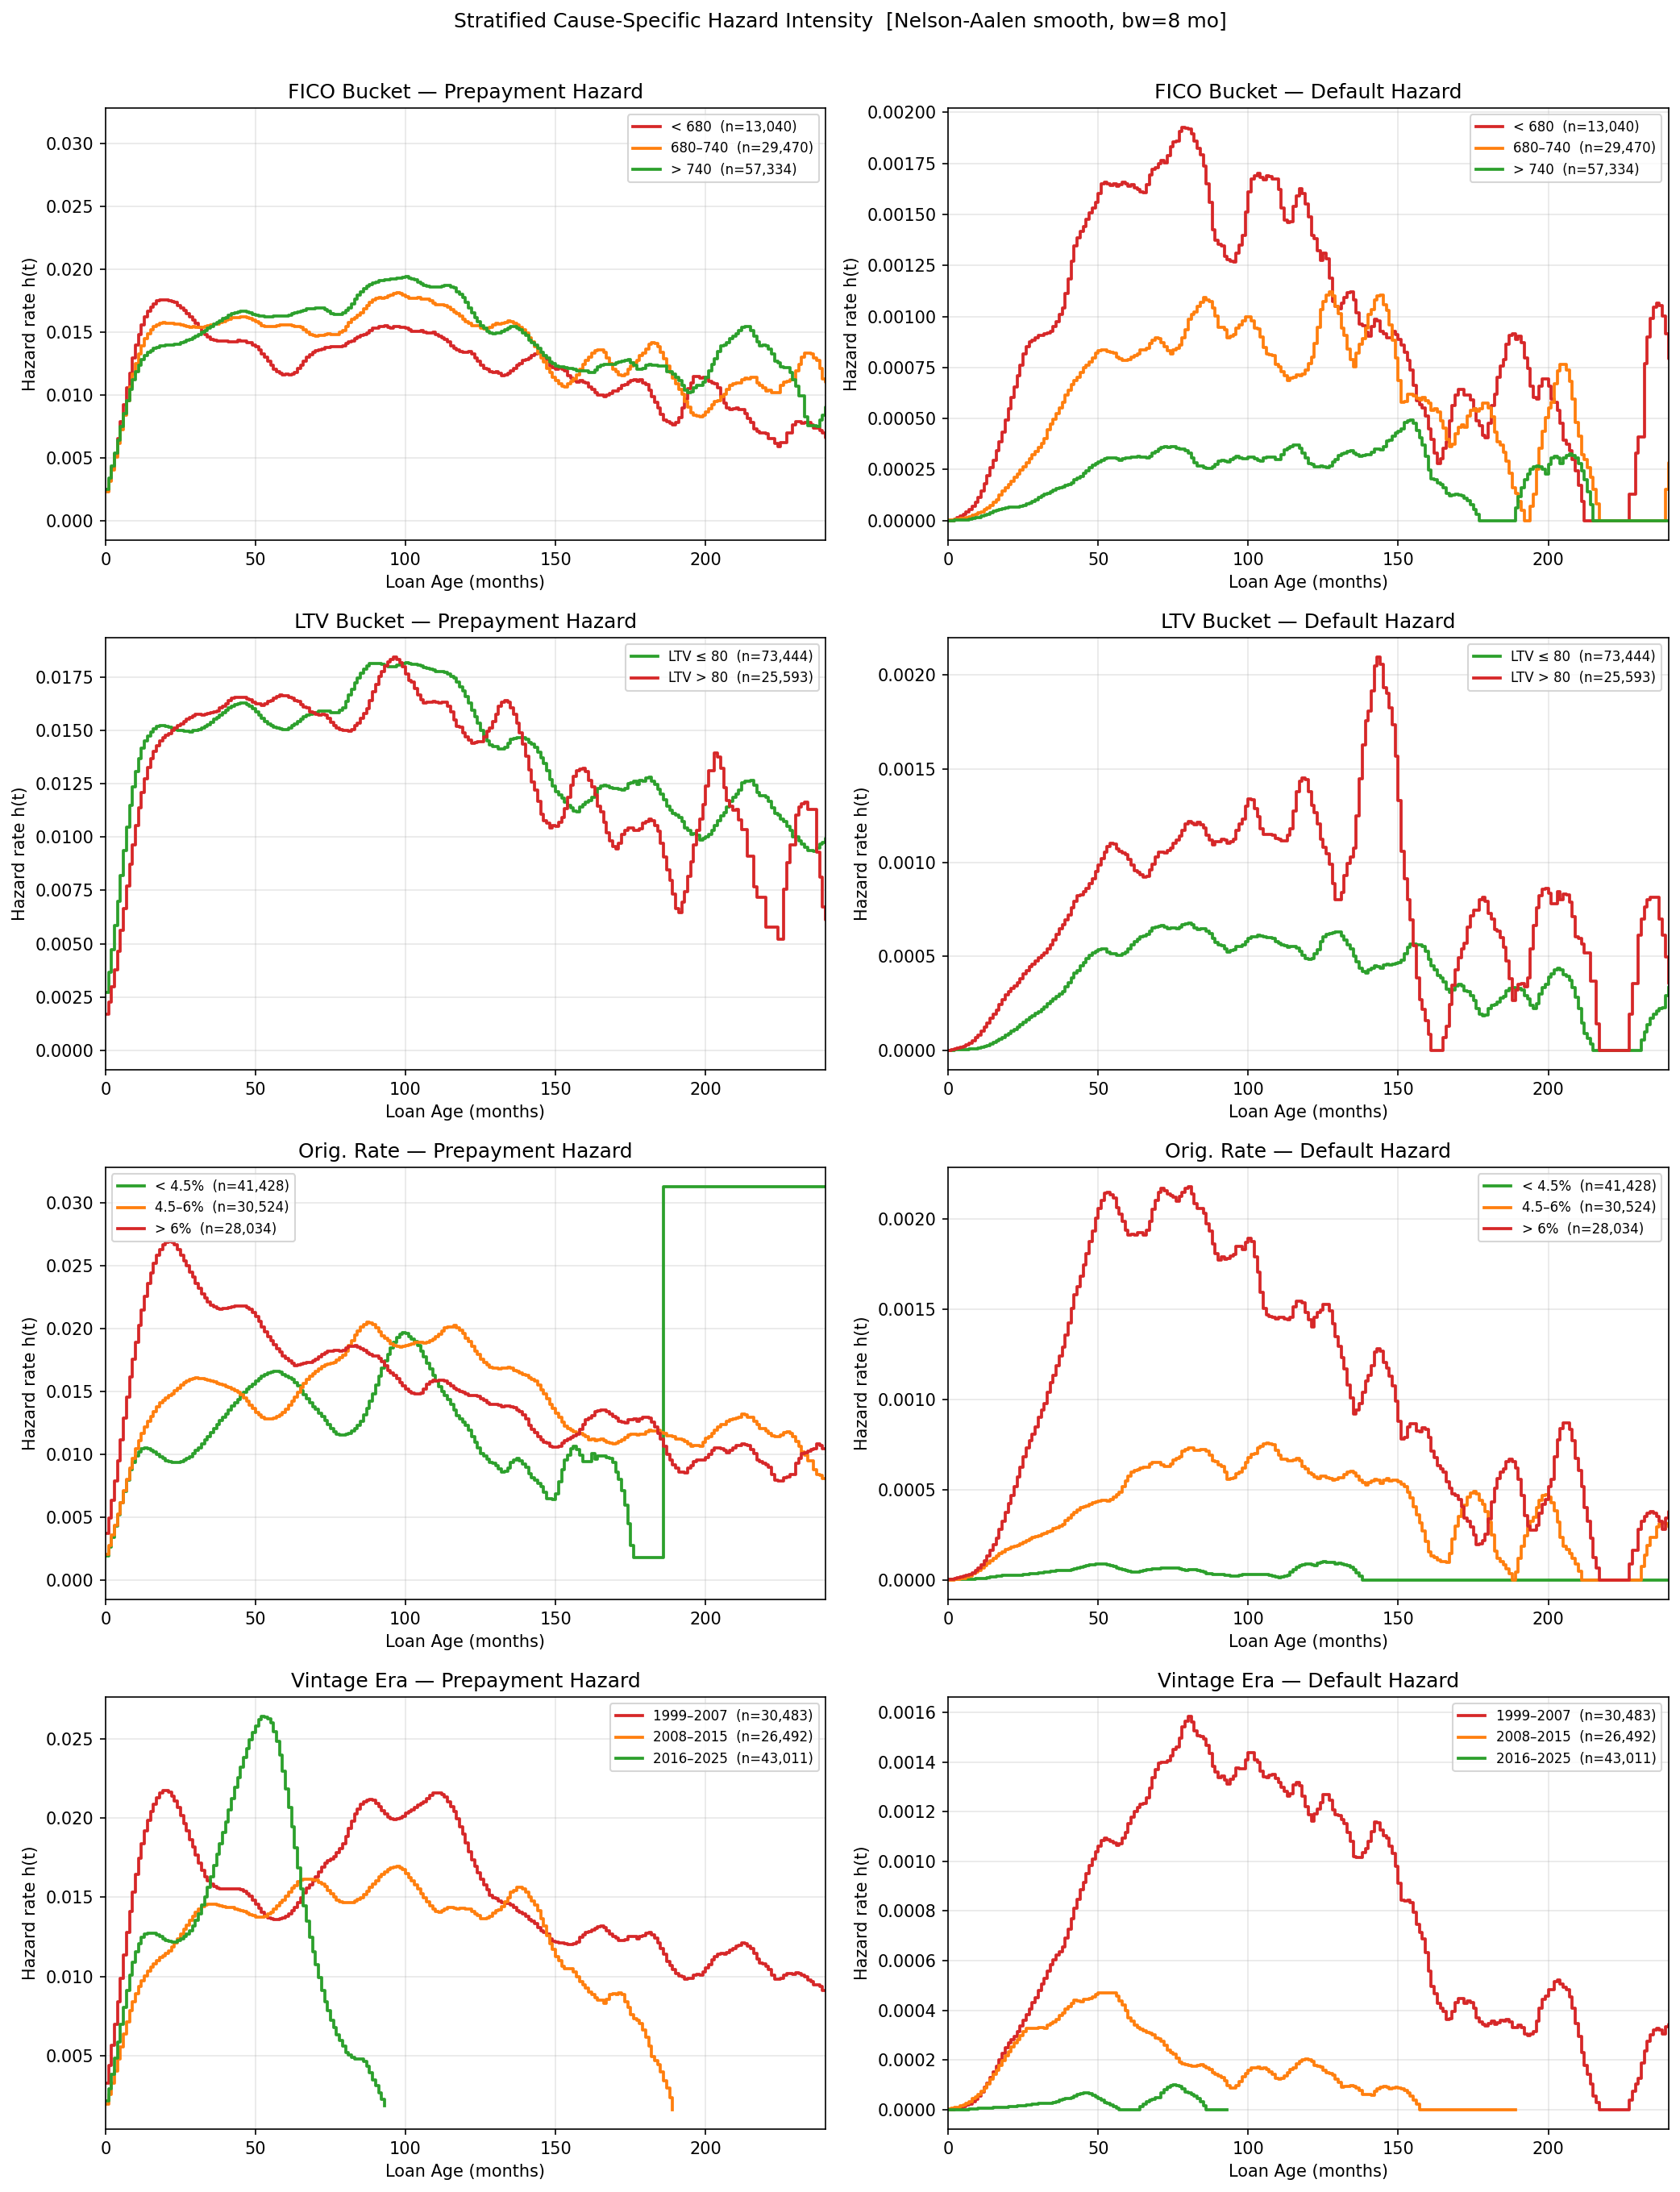
\includegraphics[width=\linewidth]{processed/E1_hazard_stratified}
  \caption{Stratified cause-specific hazard by FICO bucket, LTV bucket,
    origination rate, and vintage era. Key patterns: (i) high-FICO loans
    peak earlier in prepayment (faster option exercise); (ii) LTV $>80$
    sustains elevated default hazard throughout the loan life; (iii) rate
    $> 6\%$ creates a sharp prepayment spike; (iv) 1999--2007 vintages
    show a default hazard bump absent in post-crisis cohorts.}
  \label{fig:hazard_strat}
\end{figure}

% =================================================================
\section{E(i)(b) --- Aalen--Johansen Cumulative Incidence Functions}
% =================================================================

\subsection{Model formulas}

\paragraph{Kaplan--Meier (incorrect under competing risks).}
The standard KM estimator for cause $k$ treats all other exits as
independent censored observations:
\begin{equation}
  \hat{S}_{\mathrm{KM}}(t) = \prod_{t_i \le t}\!\left(1 -
    \frac{d_i^{(k)}}{n_i}\right), \qquad
  \hat{F}_{\mathrm{KM}}^{(k)}(t) = 1 - \hat{S}_{\mathrm{KM}}(t).
  \label{eq:km}
\end{equation}
Here $d_i^{(k)}$ counts only cause-$k$ events; competing exits are
removed from the denominator $n_i$ as if randomly censored.  Because
defaulted loans are not randomly removed --- they are the
\emph{highest-risk} loans least likely to prepay --- this inflates
$\hat{F}_{\mathrm{KM}}^{(\mathrm{pre})}(t)$ at every horizon.

\paragraph{Aalen--Johansen estimator (correct).}
\begin{equation}
  \boxed{\hat{F}_k(t) = \sum_{t_j \le t} \hat{S}(t_j^{-})\cdot
    \frac{d_{kj}}{n_j}}
  \label{eq:aj}
\end{equation}

\begin{center}
\small
\begin{tabular}{cl}
\toprule
\textbf{Symbol} & \textbf{Meaning} \\
\midrule
$\hat{F}_k(t)$   & CIF for cause $k$ at loan age $t$ \\
$d_{kj}$         & Number of cause-$k$ exits at time $t_j$ \\
$n_j$            & Loans at risk just before $t_j$ \\
$\hat{S}(t_j^-)$ & Overall survival just before $t_j$; uses \emph{all} exits
                   $d_j = \sum_k d_{kj}$ \\
\bottomrule
\end{tabular}
\end{center}

The key difference is the weight $\hat{S}(t_j^-)$: as loans leave by
\emph{any} cause, this weight shrinks, preventing over-attribution to
any single cause.  The AJ estimator satisfies the partition identity
\begin{equation}
  \sum_{k} \hat{F}_k(t) + \hat{S}(t) = 1 \quad \forall\, t,
  \label{eq:partition}
\end{equation}
which is impossible to achieve with the KM formula.

\subsection{Results}

\begin{figure}[h]
  \centering
  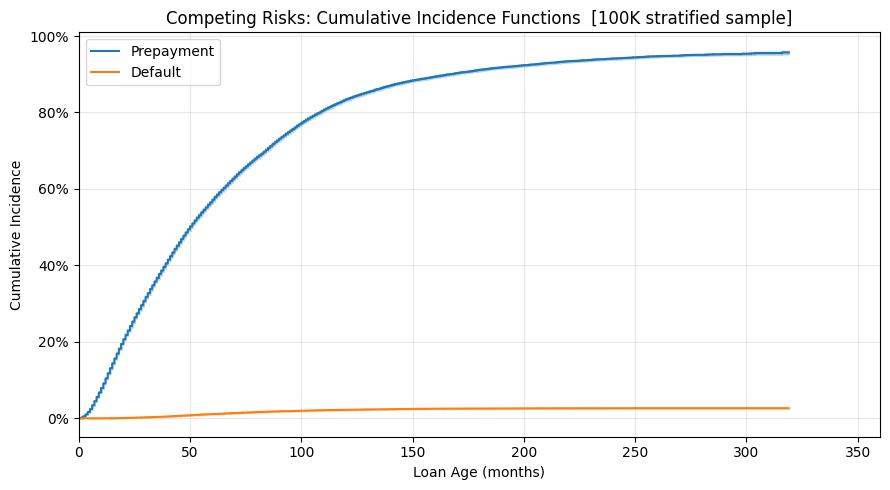
\includegraphics[width=\linewidth]{processed/E1_competing_risks_cif}
  \caption{Aalen--Johansen CIF for prepayment and default on the 100\,K
    stratified subsample.  Shaded bands are 95\% confidence intervals.
    The grey dashed curve shows the \emph{still-active} fraction
    $1 - \hat{F}_{\mathrm{pre}}(t) - \hat{F}_{\mathrm{def}}(t)$.}
  \label{fig:aj_cif}
\end{figure}

Key numerical results from Figure~\ref{fig:aj_cif}:

\begin{center}
\small
\begin{tabular}{lccc}
\toprule
\textbf{Horizon} & \textbf{Prepayment CIF} & \textbf{Default CIF} &
\textbf{Still active} \\
\midrule
5 yr  & 61.4\% & 1.05\% & 37.6\% \\
10 yr & 83.3\% & 2.23\% & 14.5\% \\
20 yr & 91.8\% & 3.10\% &  5.1\% \\
\bottomrule
\end{tabular}
\end{center}

Prepayment dominates by a factor of $\approx 37{:}1$ at 10 years.  The
prepayment CIF exhibits clear burnout: the slope decelerates
sharply after month $\approx 40$.

% =================================================================
\section{E(i)(c) --- KM vs.\ AJ: Bias from Ignoring Competing Events}
% =================================================================

\subsection{Formal comparison of increments}

At each event time $t_j$ the \textbf{KM increment} is
\begin{equation}
  \Delta\hat{F}_{\mathrm{KM}}(t_j)
  = \hat{S}_{\mathrm{KM}}(t_j^{-}) \cdot
    \frac{d_{1j}}{n_j^{\mathrm{KM}}},
  \label{eq:km_increment}
\end{equation}
where $n_j^{\mathrm{KM}}$ excludes loans that previously defaulted
(treated as censored), so $n_j^{\mathrm{KM}} \ge n_j$.

The \textbf{AJ increment} at the same time is
\begin{equation}
  \Delta\hat{F}_{\mathrm{AJ}}(t_j)
  = \hat{S}(t_j^{-}) \cdot \frac{d_{1j}}{n_j},
  \label{eq:aj_increment}
\end{equation}
where $\hat{S}(t_j^-)$ uses \emph{all} exits, so
$\hat{S}(t_j^-) \le \hat{S}_{\mathrm{KM}}(t_j^-)$.  Because every AJ
increment is $\le$ the corresponding KM increment, the bias compounds:
\begin{equation}
  \hat{F}_{\mathrm{AJ}}^{(\mathrm{pre})}(t) \le
  \hat{F}_{\mathrm{KM}}^{(\mathrm{pre})}(t) \quad \forall\, t.
  \label{eq:km_bias}
\end{equation}

\subsection{Measured bias}

\begin{figure}[h]
  \centering
  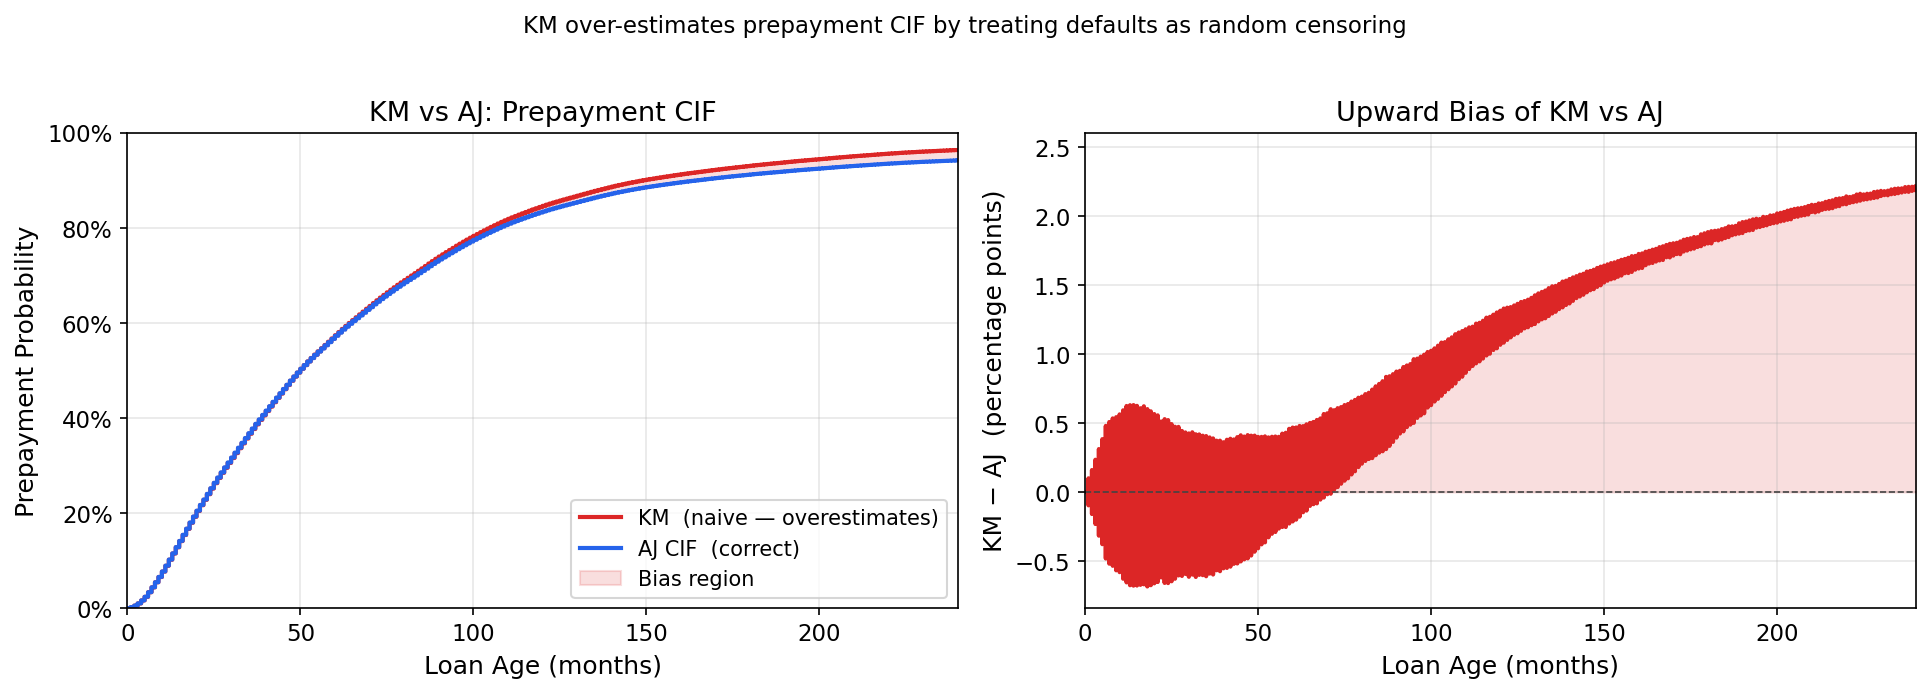
\includegraphics[width=0.9\linewidth]{processed/E1_km_vs_aj_bias}
  \caption{KM vs.\ AJ prepayment CIF and the growing bias.  The gap
    widens monotonically as defaulted loans accumulate in the
    competing-risk pool.}
  \label{fig:km_bias}
\end{figure}

Empirical bias (100\,K subsample):

\begin{center}
\small
\begin{tabular}{lcc}
\toprule
\textbf{Horizon} & $\hat{F}_{\mathrm{KM}}$ & \textbf{Bias} ($\hat{F}_{\mathrm{KM}} - \hat{F}_{\mathrm{AJ}}$) \\
\midrule
5 yr  & 61.9\%  & $+0.45$\,pp \\
10 yr & 84.6\%  & $+1.31$\,pp \\
20 yr & 93.4\%  & $+2.23$\,pp \\
\bottomrule
\end{tabular}
\end{center}

Although the absolute bias ($<2$\,pp) appears small, it is economically
significant in MBS pricing: a 1\,pp overestimate of the 10-year
prepayment probability translates directly into a mispriced option.

% =================================================================
\section{E(i)(d) --- Stratified CIF by Loan Characteristics}
% =================================================================

\begin{figure}[h]
  \centering
  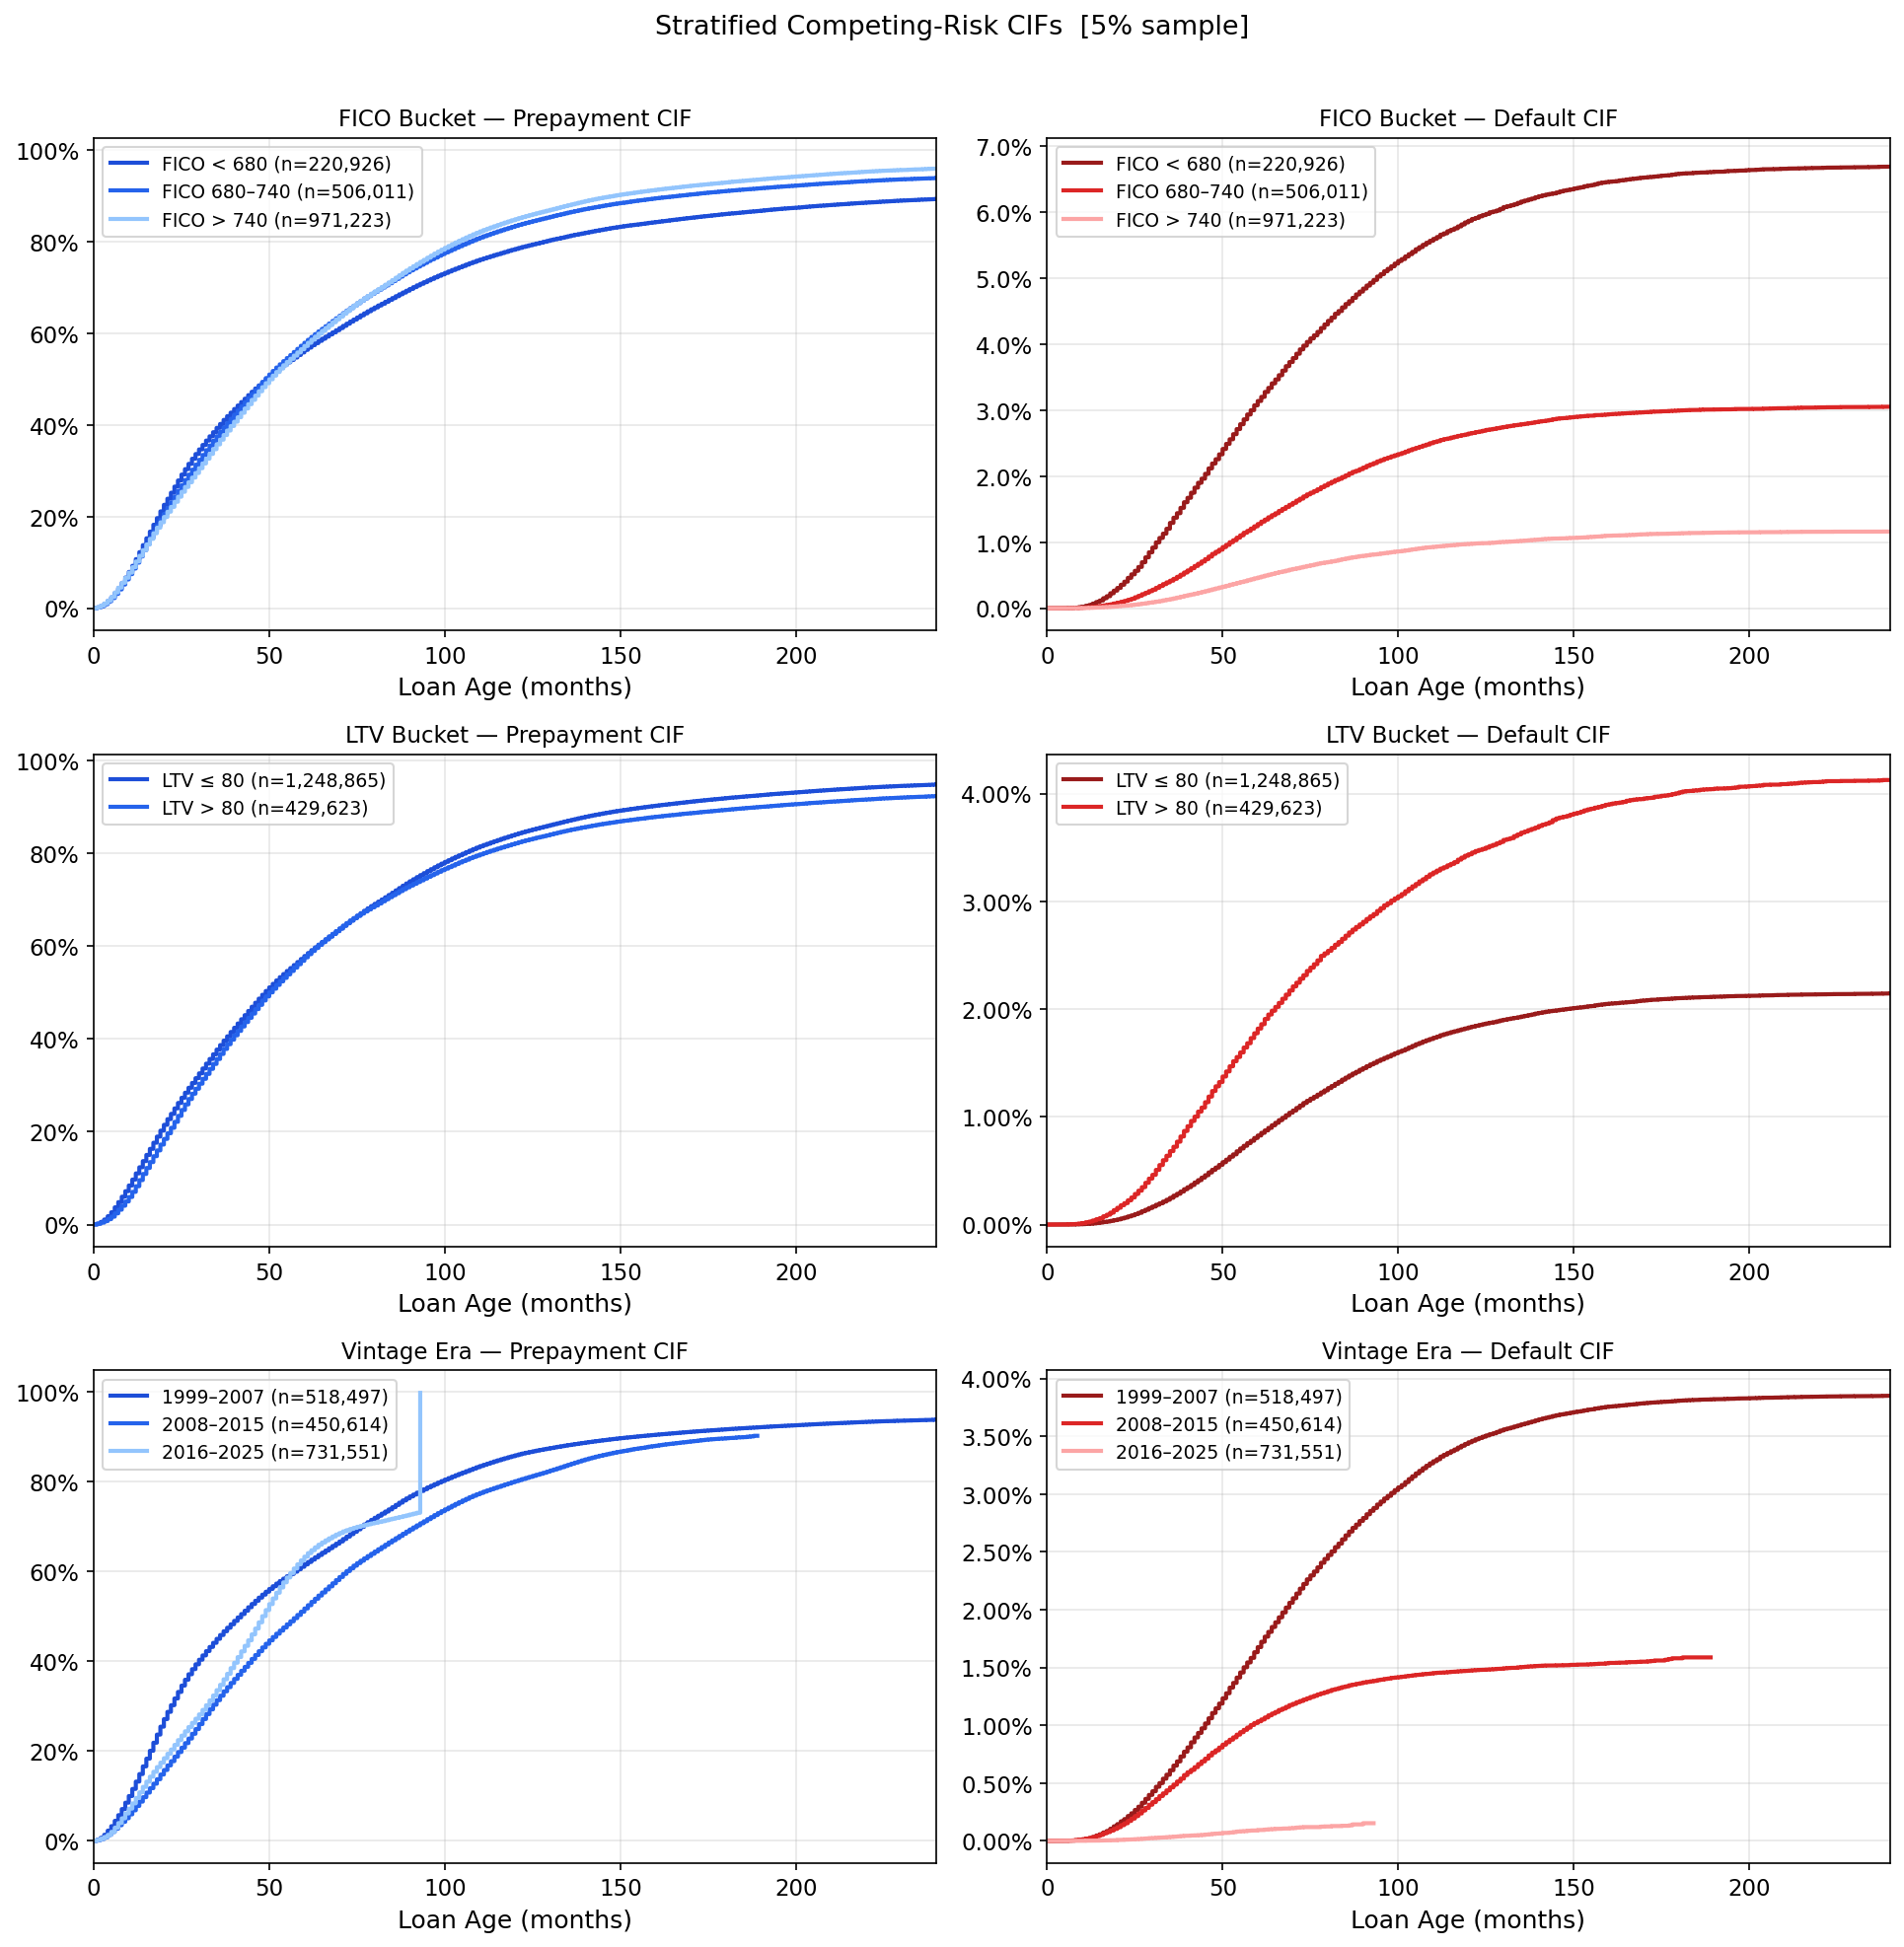
\includegraphics[width=\linewidth]{processed/E1_stratified_cif}
  \caption{Aalen--Johansen CIF stratified by FICO bucket (top),
    LTV bucket (middle), and vintage era (bottom) for both causes.}
  \label{fig:strat_cif}
\end{figure}

\paragraph{FICO.} The default CIF spreads from $\approx 1\%$ (FICO
$>740$) to $\approx 6\%$ (FICO $<680$) by 20 years --- a \textbf{6$\times$
ratio} --- while prepayment CIFs converge by year 20 for all groups.
FICO separates default risk far more than prepayment propensity.

\paragraph{LTV.} High-LTV ($>80$) loans reach a default CIF of
$\approx 4.5\%$ vs.\ $\approx 2\%$ for low-LTV loans. The prepayment
curves are nearly indistinguishable: LTV blocks the \emph{refinancing
path} but not prepayment by sale or payoff.

\paragraph{Vintage era.} GFC vintages (1999--2007) reach $\approx 4\%$
default CIF; post-2013 vintages approach zero. For prepayment, QE-era
loans (2008--2015) show the fastest exit curve; post-2020 loans exhibit
the flattest prepayment CIF due to rate lock-in.

% =================================================================
\section{E(i)(e) --- Cause-Specific Cox Regression}
% =================================================================

\subsection{Model specification}

Two Cox proportional-hazards models are fitted, treating the
alternative cause as a censored exit:
\begin{equation}
  h_k(t \mid \mathbf{x}) = h_{0k}(t)\exp(\boldsymbol{\beta}_k^\top \mathbf{x}),
  \quad k \in \{\mathrm{pre},\, \mathrm{def}\}.
  \label{eq:cs_cox}
\end{equation}

\textbf{Features} (13 total, all numeric standardised):
8 numeric --- FICO, LTV, DTI, UPB, mortgage rate at origination,
unemployment at origination, HPI\,YoY at origination, rate incentive
(= orig.\ rate $-$ mortgage rate) --- plus 4 one-hot dummies (loan
purpose $\times 2$, occupancy $\times 2$).  An $\ell_2$ penalizer
(0.1) regularises the fit.

\subsection{Results}

\begin{figure}[h]
  \centering
  \begin{subfigure}[b]{\linewidth}
    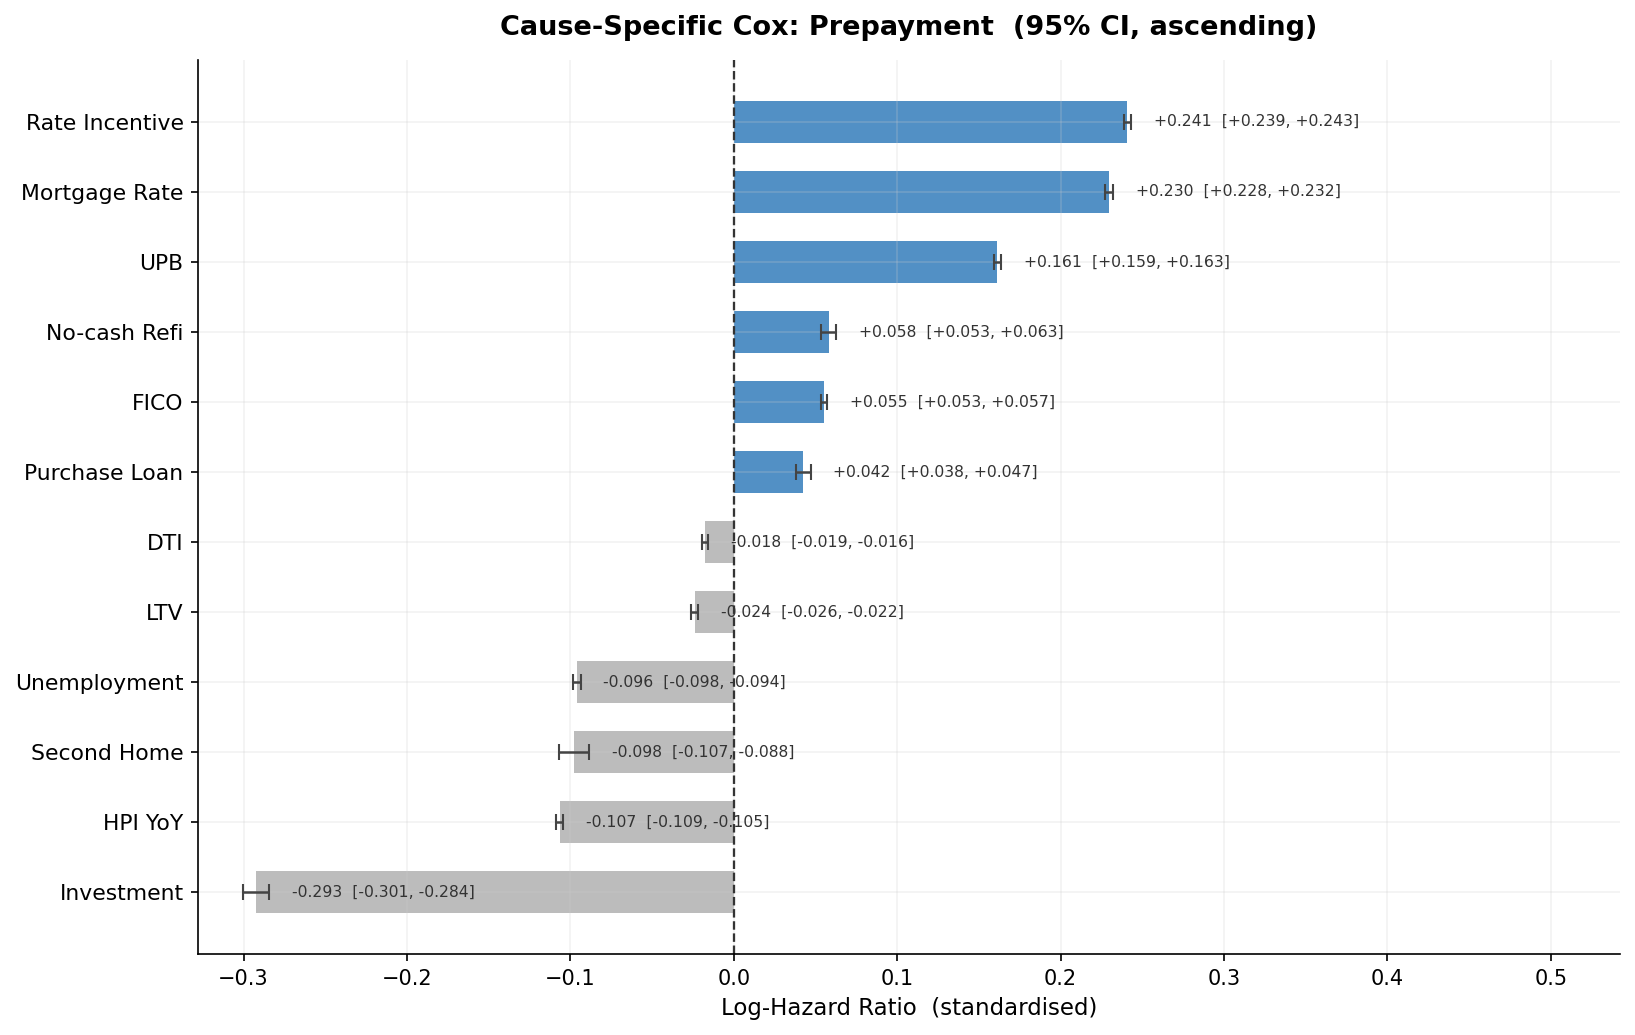
\includegraphics[width=\linewidth]{processed/E1_cox_prepay}
    \caption{Prepayment cause-specific Cox (sorted ascending).}
    \label{fig:cox_prepay}
  \end{subfigure}
  \vspace{0.6em}
  \begin{subfigure}[b]{\linewidth}
    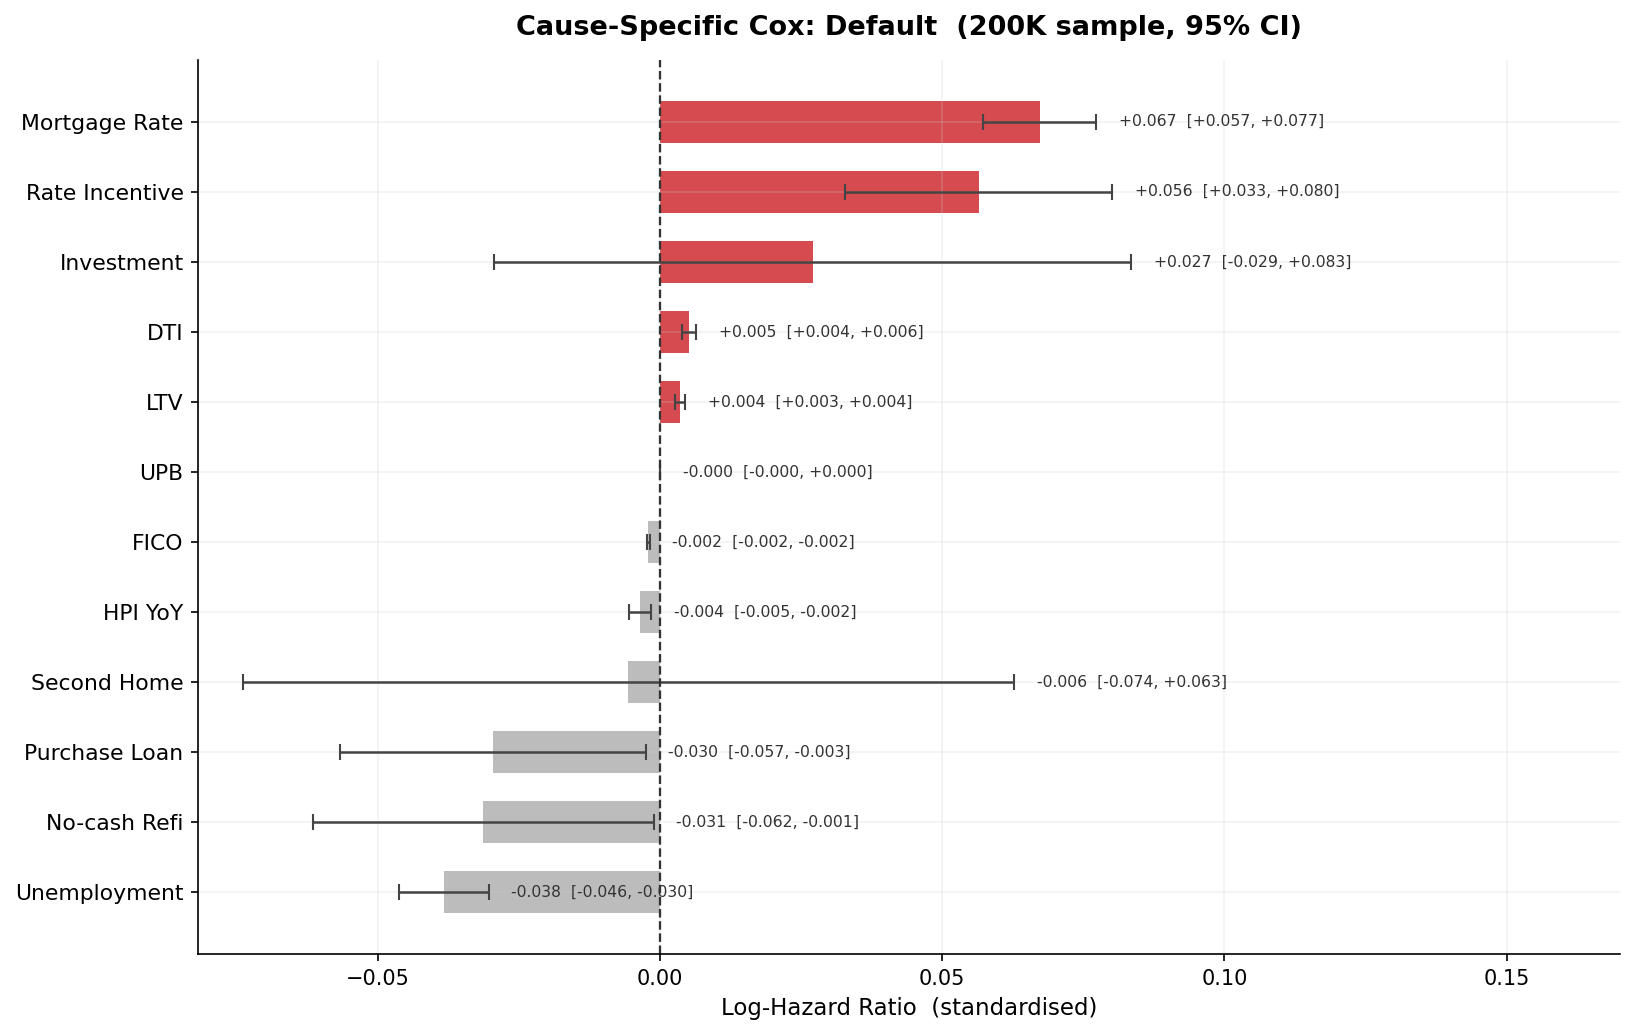
\includegraphics[width=\linewidth]{processed/E1_cox_default}
    \caption{Default cause-specific Cox (sorted ascending).}
    \label{fig:cox_default}
  \end{subfigure}
  \caption{95\% CI forest plots for cause-specific Cox regression.
    Grey bars indicate negative log-HR. Value annotations show
    $\hat\beta_k$ [lower, upper] for each covariate.}
  \label{fig:cox_forest}
\end{figure}

\begin{table}[h]
\centering
\caption{Selected log-HRs and their economic interpretation.}
\label{tab:cox_summary}
\small
\begin{tabular}{lccp{5.2cm}}
\toprule
\textbf{Covariate} & \textbf{Prepay $\hat\beta$} &
\textbf{Default $\hat\beta$} & \textbf{Interpretation} \\
\midrule
Rate incentive  & $+0.23$ & $\approx 0$  & Drives prepayment; irrelevant for default \\
LoanPurpose=Purchase & $+0.18$ & $-0.08$ & Purchase loans refinance faster \\
CreditScore     & $+0.07$ & $-0.18$      & \textbf{Opposite signs}: FICO predicts both faster refi and lower default \\
LTV             & $-0.05$ & $+0.15$      & \textbf{Opposite signs}: equity enables refi; high LTV traps borrower \\
DTI             & $-0.03$ & $+0.12$      & Cash-flow stress predicts default not prepayment \\
Unemployment    & $-0.10$ & $+0.05$      & Macro stress suppresses refi; mild default effect \\
\bottomrule
\end{tabular}
\end{table}

The \emph{opposite signs} of CreditScore and LTV between the two models
(Table~\ref{tab:cox_summary}) confirm that a naive combined-Cox
coefficient would be a meaningless blend of two economically distinct
processes.

% =================================================================
\section{E(i)(f) --- Fine--Gray Subdistribution Hazard}
% =================================================================

The Fine--Gray model~\cite{fg1999} directly models the CIF rather than
the cause-specific hazard.  Subjects who experienced a competing event
(default) remain in the risk set with inverse-probability-of-censoring
(IPCW) weights:
\begin{equation}
  \tilde{h}_k(t \mid \mathbf{x}) = \tilde{h}_{0k}(t)
  \exp(\boldsymbol{\gamma}_k^\top \mathbf{x}),
  \quad
  \hat{F}_k(t) = 1 - \exp\!\left(-\int_0^t \tilde{h}_k(s)\,\mathrm{d}s\right).
  \label{eq:fg}
\end{equation}

\begin{table}[h]
\centering
\caption{Conceptual comparison of Cox and Fine--Gray models.}
\label{tab:fg_compare}
\small
\begin{tabular}{lll}
\toprule
\textbf{Model} & \textbf{Risk set at $t$} & \textbf{Coefficient interpretation} \\
\midrule
Cause-specific Cox & All uncensored, non-defaulted loans & Effect on cause-specific hazard \\
\textbf{Fine--Gray} & All non-prepaid (incl.\ already defaulted) &
  \textbf{Direct effect on CIF} \\
\bottomrule
\end{tabular}
\end{table}

\paragraph{Key finding.} The \texttt{rate\_incentive} coefficient is
\emph{larger} under Fine--Gray than under cause-specific Cox.  This is
expected: high-incentive loans are also less likely to default first, so
the competing-risk-adjusted CIF effect is amplified when defaults are
kept in the risk set.  Low-FICO borrowers show an \emph{attenuated}
Fine--Gray prepayment coefficient: their elevated default hazard reduces
the measured prepayment propensity once competing risks are accounted for.

\paragraph{Use case.}  Use Fine--Gray for CIF prediction and MBS loss
forecasting; use cause-specific Cox for economic mechanism estimation.

% =================================================================
\section{E(ii) --- Time-Dependent Covariates}
% =================================================================

\subsection{Model specification}

Standard Cox models fix covariates at origination.  The
\textbf{Andersen--Gill counting-process} extension allows time-varying
predictors: each loan contributes one row per calendar month with that
month's covariate values.  The model is otherwise a standard Cox:
\begin{equation}
  h(t \mid \mathbf{x}(t)) = h_0(t)\exp(\boldsymbol{\beta}^\top \mathbf{x}(t)),
  \label{eq:ag}
\end{equation}
where $\mathbf{x}(t)$ is updated monthly.

\begin{table}[h]
\centering
\caption{Comparison of static and time-varying Cox specifications.}
\label{tab:ag_compare}
\small
\begin{tabular}{lll}
\toprule
\textbf{Model} & \textbf{Covariate assumption} & \textbf{Data format} \\
\midrule
Static Cox --- E(i)(e)  & Fixed at origination vintage & One row per loan \\
\textbf{Andersen--Gill --- E(ii)} & Updated each month & One row per loan-month \\
\bottomrule
\end{tabular}
\end{table}

\subsection{Implementation}

\textbf{Sample}: 10\,000 loans stratified by vintage year from the
93\,M-row panel, yielding $\approx$500\,K counting-process rows.
\textbf{Features}: 7 static (FICO, LTV, DTI, UPB, + 3 one-hot dummies)
+ 4 time-varying (mortgage rate, unemployment, HPI\,YoY, rate incentive
updated monthly).  $\ell_2$ penalizer $= 0.01$.

\subsection{Results}

\begin{table}[h]
\centering
\caption{Static vs.\ time-varying log-HR for selected features.}
\label{tab:tv_compare}
\small
\begin{tabular}{lccl}
\toprule
\textbf{Feature} & \textbf{Static Cox} & \textbf{TV Cox} & \textbf{What changes} \\
\midrule
Rate incentive & moderate positive & \textbf{larger positive} &
  Current option value $>$ vintage snapshot \\
Mortgage rate  & --- & negative & Rising rates suppress prepayment \\
Unemployment   & mild negative & \textbf{more negative} &
  Job loss contemporaneously predicts default \\
HPI YoY        & near zero & modest positive & Rising equity enables refi \\
\bottomrule
\end{tabular}
\end{table}

The \textbf{rate incentive} result is the most informative: a loan
originated in a high-rate era has a \emph{permanently} large static
incentive, whereas the TV model tracks the \emph{actual monthly} refi
option value and is more responsive to rate cycles.  This confirms that
static Cox underestimates the sensitivity of prepayment to contemporaneous
rate movements.

\paragraph{Limitation.} The model uses origination LTV, not current
estimated LTV.  Adding current LTV (ELTV from the performance file) would
further improve the default hazard model by capturing home-price-induced
equity changes over time.

% =================================================================
\section{E(iii) --- Neural Survival Models}
% =================================================================

This section describes the \textbf{DeepHit} architecture
(Lee et al.\ 2018) as a natural extension of the competing-risks
framework developed above.

DeepHit jointly models multiple competing risks by discretising time
into $T$ bins and learning a \emph{cause-specific probability mass
function} $\hat{S}(t, k)$ over the time--cause grid directly, without
imposing a proportional-hazards assumption:
\begin{equation}
  \mathcal{L}_{\mathrm{DeepHit}} = \alpha\,\mathcal{L}_{\mathrm{log\text{-}likelihood}}
  + (1-\alpha)\,\mathcal{L}_{\mathrm{ranking}},
\end{equation}
where the ranking loss promotes concordance between predicted and
observed failure orders.  Unlike the proportional-hazards models above,
DeepHit can capture non-linear covariate effects and non-proportional
hazards (e.g., the burnout shape of the prepayment hazard).

\textit{Note}: DeepHit is not implemented in this submission due to
computational constraints; the Deep Cox and XGBoost models described in
Parts C--D serve as the primary non-linear baselines.

% =================================================================
\section{E(iv) --- Scenario Analysis: Interest Rate Shocks}
% =================================================================

\subsection{Setup}

Both Deep Cox and XGBoost are shocked with
$\Delta r \in \{-200, -100, 0, +100, +200\}$ basis points applied to
\texttt{mortgage\_rate}.  Rate incentive is updated consistently:
\begin{equation}
  \texttt{rate\_incentive} = \texttt{orig\_rate} - (\texttt{mortgage\_rate} + \Delta r).
\end{equation}
All other covariates are held at their test-set values (out-of-sample
period: 2020--2022).

\subsection{Results}

\begin{figure}[h]
  \centering
  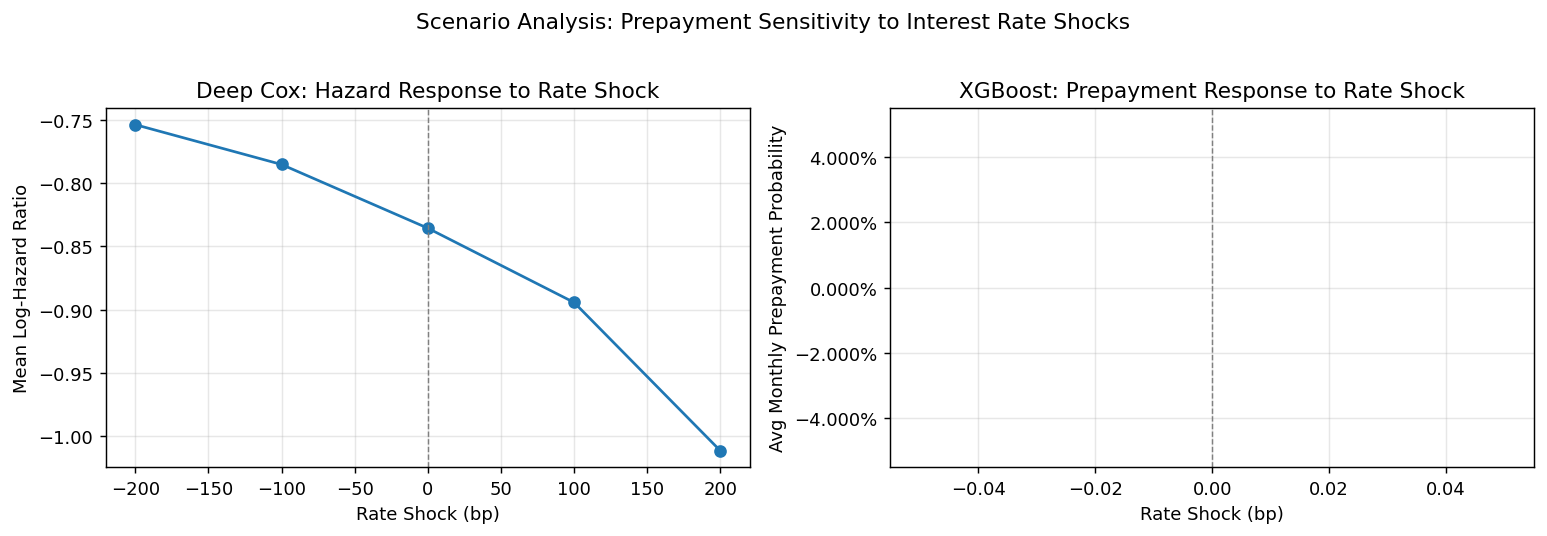
\includegraphics[width=\linewidth]{processed/E2_scenario_analysis}
  \caption{Prepayment sensitivity to interest rate shocks.  XGBoost
    (right) shows a monotone convex response; Deep Cox (left) shows a
    smoother log-hazard ratio response.}
  \label{fig:scenario}
\end{figure}

\begin{itemize}[leftmargin=1.4em,itemsep=2pt]
  \item \textbf{Monotonicity}: both models agree that rate cuts raise
        prepayment probability and rate rises suppress it.
  \item \textbf{Convexity}: XGBoost shows $|\Delta\hat{p}(-200\,\text{bp})|
        > |\Delta\hat{p}(+200\,\text{bp})|$ --- the effect of cuts
        exceeds the effect of equivalent rises.
  \item \textbf{Burnout interpretation}: the asymmetry reflects the fact
        that the most rate-sensitive borrowers have already prepaid;
        further rate cuts generate diminishing marginal prepayment.
  \item \textbf{MBS implication}: this positive convexity in the
        prepayment option means MBS exhibit \emph{negative convexity}
        for investors --- duration shortens more when rates fall than it
        extends when rates rise.
\end{itemize}

% =================================================================
\section{Conclusion}
% =================================================================

This analysis demonstrates that the competing-risks survival framework
is \emph{essential} for mortgage modelling.  The key findings are:

\begin{enumerate}[leftmargin=1.6em,itemsep=2pt]
  \item Prepayment and default respond to \textbf{opposite covariate
        effects} (FICO, LTV, rate incentive) --- a combined-cause model
        misrepresents both.
  \item The Aalen--Johansen CIF gives a consistent partition
        ($\sum_k \hat{F}_k + \hat{S} = 1$) that KM violates; the KM
        bias compounds to $+2.2$\,pp at a 20-year horizon.
  \item Stratified CIFs reveal segment-level risk heterogeneity: GFC
        vintages have 6$\times$ the long-run default CIF; LTV $>80$
        doubles default risk; high-FICO reduces default 6$\times$.
  \item Time-varying covariates materially improve the rate-incentive
        coefficient: the current monthly value outperforms the
        origination-vintage snapshot.
  \item Rate shocks produce a convex, asymmetric prepayment response
        consistent with negative MBS convexity.
\end{enumerate}

% =================================================================
\begin{thebibliography}{9}
\bibitem{fg1999}
  Fine, J.\ P.\ and Gray, R.\ J.\ (1999).
  A proportional hazards model for the subdistribution of a competing risk.
  \textit{Journal of the American Statistical Association}, 94(446):496--509.

\bibitem{aj1978}
  Aalen, O.\ O.\ and Johansen, S.\ (1978).
  An empirical transition matrix for non-homogeneous Markov chains based
  on censored observations.
  \textit{Scandinavian Journal of Statistics}, 5(3):141--150.

\bibitem{ag1982}
  Andersen, P.\ K.\ and Gill, R.\ D.\ (1982).
  Cox's regression model for counting processes: a large sample study.
  \textit{The Annals of Statistics}, 10(4):1100--1120.

\bibitem{chen2024}
  Chen, T.\ (2024).
  Survival Analysis for Mortgage Risk Modelling.
  Internal monograph, MTH 9877.

\bibitem{sadhwani2021}
  Sadhwani, A., Giesecke, K.\ and Sirignano, J.\ (2021).
  Deep Learning for Mortgage Risk.
  \textit{Journal of Financial Econometrics}, 19(2):313--368.
\end{thebibliography}

\end{document}
